\documentclass[a4paper, 12pt]{article}
\usepackage[a4paper,top=1.3cm,bottom=2cm,left=1.5cm,right=1.5cm,marginparwidth=0.75cm]{geometry}
\usepackage{wrapfig}
\usepackage{graphicx}
\usepackage{mathtext}
\usepackage{amsmath}
\usepackage{siunitx}
\usepackage{subfigure}
\usepackage{multirow}
\usepackage{rotating}
\usepackage[T1,T2A]{fontenc}
\usepackage[russian]{babel}
\usepackage{caption}

\graphicspath{{pictures/}}
\begin{document}

\pagenumbering{gobble}
\pagenumbering{arabic}

\title{\textbf{Измерение вязкости воздуха по течению в тонких трубках. (1.3.3)}}
\author{Зайнуллин Амир Б05-206}
\maketitle

\section{Аннотация}
    \textbf{Цель работы:} экспериментально исследовать свойства течения газов по тонким трубкам при различных числах Рейнольдса; выявить область применимости закона Пуазейля и с его помощью определить коэффициент вязкости воздуха. \\
	\textbf{Оборудование:} система подачи воздуха (компрессор, поводящие трубки); газовый счетчик барабанного типа; спиртовой микроманометр с регулируемым наклоном; набор трубок различного диаметра с выходами для подсоединения микроманометра; секундомер.

\section{Теоретические сведения}
    Сила вязкого трения согласно закону Ньютона, где $\eta$ это коэффициент динамической вязкости (или просто вязкость среды):
    \begin{equation}
        \tau = \eta \frac{\partial \upsilon_x}{\partial y}
    \end{equation}

    Характер течения в жидкости может быть турбулентным или ламинарным. При ламинарном течении скорости образуют набор непрерывных линий тока, а слои жидкости не перемешиваются между собой. При малых $Re$ течение ламирно. 
    \begin{equation}
        Re = \frac{\rho u a}{\eta}
    \end{equation} 
    $\rho$ - плотность среды, $u$ - характерная скорость потока, $a$ - характерный размер системы.
        
    \medskip

    Формула Пуазейля:
    \begin{equation}
        Q = \frac{\pi R^4\Delta P}{8\eta l} \hspace*{20mm} \bar{u} = \frac{Q}{\pi R^2} \text{    - средняя скорость потока}
    \end{equation}

    Длина установления течения Пуазейля:
    \begin{equation}
        l_{уст} \approx 0.2R\cdot Re
    \end{equation}

    Отношение перепада давления в трубе к скоростному напору:
    \begin{equation}
        \tilde{\psi} = \frac{R}{l}\frac{\Delta P}{\rho \bar{u}^2}
    \end{equation}

    Из теории размерностей:
    \begin{equation}
        \frac{\Delta P}{l} = C(Re)\cdot \frac{\rho \bar{u}^2}{R}
    \end{equation}

    При больших числах Рейнольдса параметры течения жидкости не зависят от коэффициента вязкости, поэтому $C(Re)\mapsto const$, oткуда
    \begin{equation}
        Q = const \cdot R^{5/2} \sqrt{\frac{\Delta P}{\rho l}}
    \end{equation}


\section{Экспериментальная установка}
    \begin{figure}[!ht]
        \center{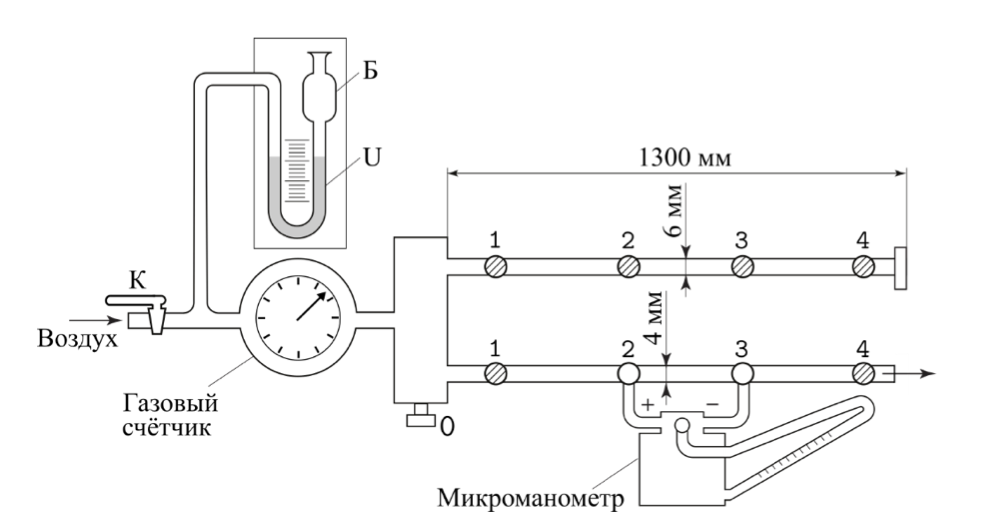
\includegraphics[width=0.8\textwidth]{ustanovka.png}}
        \caption{Экспериментальная установка}
    \end{figure}
    Поток воздуха под давлением немного превышающим атмосферное, поступает через газовый счетчик в тонкие металлические трубки. Интенсивность его подачи регулируется краном К. \par 
    U-образный манометр для измерения давления на входе.
    
    В работе используется газовый счётчик барабанного
    типа, позволяющий измерять объём газа $\Delta V$ прошедшего через систему. Измеряя время $\Delta t$ при помощи секундомера, можно вычислить средний объёмный расход газа $Q = \Delta V/ \Delta t$ (для получения массового расхода [кг/с] результат
    необходимо домножить на плотность газа $\rho$). \par 
    Разность давлений на входах манометра измеряется по высоте подъема рабочей жидкости.

    \subsection*{Инструментальные погрешности}

     {\bf Газовый счётчик: } класс точности 1 \\
     {\bf Микроманометр: } класс точности 1 \\
     {\bf Секундомер: } $\Delta = \pm 0.3 $ с

\section{Результаты измерений и обработка данных}

Измерили параметры окружающей среды: температуру, влажность воздуха и атмосферное давление. 

\begin{table}[!ht]
    \centering
    \begin{tabular}{|c|c|c|}
    \hline
        P, кПа & $T, К$  & $\varphi, \%$  \\ \hline
        98.5 & 294,5 & 18.5  \\ \hline
    \end{tabular}
    \caption{Параметры окружающей среды}
\end{table}

Проведем предварительные расчеты по следующим формулам. $ \eta = 2 \cdot 10^{-5} \text{ Па} \cdot \text{c} $ , $Re = 1000$
\[ \rho  = \dfrac{pM}{RT} \] 
\[ Q_{\text{кр}} = \frac{Re  \eta  \pi  r  R  T }{p  M} \]
\[ \Delta P_{\text{кр}} = \frac{8Q_{\text{кр}} \eta l}{\pi r^4} \]

\begin{table}[!ht]
    \centering
    \begin{tabular}{|c|c|c|c|}
    \hline
        $l$, см & 50 & 90 & 40 \\ \hline
        $d$, мм & 3,95 & 4,95 & 3 \\ \hline
        Из теории & ~ & ~ & ~ \\ \hline
        $Q_{кр} \cdot 10^{-4} \text{ }\dfrac{\text{м} ^ 3}{\text{c}}$ & 1,06 & 1,36 & 0,82 \\ \hline
        $p_{кр}$, Па& 178 & 153 & 328 \\ \hline
        $p_{кр}$, дел. & 91 & 71 & 169 \\ \hline
        l, см & 39,5 & 50,5 & 34,2 \\ \hline
        из эксп. & ~ & ~ & ~ \\ \hline
        $p_{кр}$, дел. & 75 & 65 & 168 \\ \hline
    \end{tabular}
    \caption{Полученные данные}
\end{table}

Подобрали параметры измерения так, чтобы относительная погрешность была меньше процента. Для малых давлений относительная погрешность больше процента, потому что объем измерялся долго.
Абсолютная погрешность измерения объема равна $5 \text{ л} \cdot 0,01 = 0,05 \text{ л}$, так как класс точности газового счетчика равен 1, а предел измерения равен $5$ л.

\begin{table}[!ht]
    \centering
    \begin{tabular}{|c|c|c|c|c|c|c|c|}
    \hline
        $t$, c & $\varepsilon_T$ & $V$, л & $\varepsilon_V$ & $\Delta$P, мм & P, Па & Q, м$^3$/c $\cdot$ 10$^{-4}$ & $\sigma_Q$, м$^3$/c $\cdot$ 10$^{-4}$ \\ \hline
        166 & 0,0002 & 4 & 0,013 & 20 & 39 & 0,24 & 0,003 \\ \hline
        113,3 & 0,0003 & 4 & 0,013 & 29 & 57 & 0,35 & 0,005 \\ \hline
        140,4 & 0,0002 & 6 & 0,008 & 35 & 68 & 0,43 & 0,004 \\ \hline
        137 & 0,0002 & 7 & 0,007 & 42 & 82 & 0,51 & 0,004 \\ \hline
        115,6 & 0,0003 & 7 & 0,007 & 50 & 98 & 0,61 & 0,004 \\ \hline
        113,3 & 0,0003 & 8 & 0,006 & 58 & 113 & 0,71 & 0,005 \\ \hline
        99,1 & 0,0003 & 8 & 0,006 & 66 & 129 & 0,81 & 0,005 \\ \hline
        89,9 & 0,0003 & 8 & 0,006 & 72 & 141 & 0,89 & 0,006 \\ \hline
        82,1 & 0,0004 & 8 & 0,006 & 92 & 180 & 0,97 & 0,006 \\ \hline
        76,1 & 0,0004 & 8 & 0,006 & 120 & 235 & 1,05 & 0,007 \\ \hline
        69,9 & 0,0004 & 8 & 0,006 & 148 & 290 & 1,14 & 0,008 \\ \hline
        74,8 & 0,0004 & 9 & 0,006 & 166 & 325 & 1,20 & 0,007 \\ \hline
        71,2 & 0,0004 & 9 & 0,006 & 185 & 362 & 1,26 & 0,008 \\ \hline
        63 & 0,0005 & 9 & 0,006 & 235 & 460 & 1,43 & 0,009 \\ \hline
        58 & 0,0005 & 9 & 0,006 & 275 & 538 & 1,55 & 0,009 \\ \hline
    \end{tabular}
    \caption{Таблица измерений для $3,95$ мм }
\end{table}

\begin{table}[!ht]
    \centering
    \begin{tabular}{|c|c|c|c|c|c|c|c|}
    \hline
    $t$, c & $\varepsilon_T$ & $V$, л & $\varepsilon_V$ & $\Delta$P, мм & P, Па & Q, м$^3$/c $\cdot$ 10$^{-4}$ & $\sigma_Q$, м$^3$/c $\cdot$ 10$^{-4}$ \\ \hline
    111,1 & 0,0003 & 6 & 0,008 & 26 & 51 & 0,54 & 0,005 \\ \hline
    93,5 & 0,0003 & 6 & 0,008 & 31 & 61 & 0,64 & 0,006 \\ \hline
    76,3 & 0,0004 & 6 & 0,008 & 39 & 76 & 0,79 & 0,007 \\ \hline
    76,2 & 0,0004 & 7 & 0,007 & 47 & 92 & 0,92 & 0,007 \\ \hline
    77,4 & 0,0004 & 8 & 0,006 & 54 & 106 & 1,03 & 0,007 \\ \hline
    72 & 0,0004 & 8 & 0,006 & 60 & 117 & 1,11 & 0,007 \\ \hline
    69,4 & 0,0004 & 8 & 0,006 & 66 & 129 & 1,15 & 0,008 \\ \hline
    59,3 & 0,0005 & 8 & 0,006 & 90 & 176 & 1,35 & 0,009 \\ \hline
    51,6 & 0,0006 & 8 & 0,006 & 127 & 248 & 1,55 & 0,011 \\ \hline
    53,8 & 0,0006 & 9 & 0,006 & 153 & 299 & 1,67 & 0,010 \\ \hline
    49,8 & 0,0006 & 9 & 0,006 & 175 & 342 & 1,81 & 0,011 \\ \hline
    46,1 & 0,0007 & 9 & 0,006 & 205 & 401 & 1,95 & 0,012 \\ \hline
    42,5 & 0,0007 & 9 & 0,006 & 238 & 466 & 2,12 & 0,013 \\ \hline
    40,4 & 0,0007 & 9 & 0,006 & 262 & 513 & 2,23 & 0,014 \\ \hline
    \end{tabular}
    \caption{Таблица измерений для $5,05$ мм }
\end{table}

\newpage

\begin{table}[!ht]
    \centering
    \begin{tabular}{|c|c|c|c|c|c|c|c|}
    \hline
        $t$, c & $\varepsilon_T$ & $V$, л & $\varepsilon_V$ & $\Delta$P, мм & P, Па & Q, м$^3$/c $\cdot$ 10$^{-4}$ & $\sigma_Q$, м$^3$/c $\cdot$ 10$^{-4}$ \\ \hline
        68,6 & 0,0004 & 3 & 0,017 & 40 & 78 & 0,44 & 0,007 \\ \hline
        71 & 0,0004 & 4 & 0,013 & 55 & 108 & 0,56 & 0,007 \\ \hline
        59,4 & 0,0005 & 4 & 0,013 & 74 & 145 & 0,67 & 0,009 \\ \hline
        66 & 0,0005 & 5 & 0,010 & 90 & 176 & 0,76 & 0,008 \\ \hline
        63,7 & 0,0005 & 6 & 0,008 & 125 & 245 & 0,94 & 0,008 \\ \hline
        53,1 & 0,0006 & 6 & 0,008 & 170 & 333 & 1,13 & 0,010 \\ \hline
        59,6 & 0,0005 & 7 & 0,007 & 195 & 382 & 1,17 & 0,009 \\ \hline
        52,3 & 0,0006 & 7 & 0,007 & 229 & 448 & 1,34 & 0,010 \\ \hline
        57,9 & 0,0005 & 8 & 0,006 & 252 & 493 & 1,38 & 0,009 \\ \hline
        55,9 & 0,0005 & 8 & 0,006 & 275 & 538 & 1,43 & 0,010 \\ \hline
    \end{tabular}
    \caption{Таблица измерений для $3$ мм }
\end{table}


\begin{figure}[!ht]
    \centering
    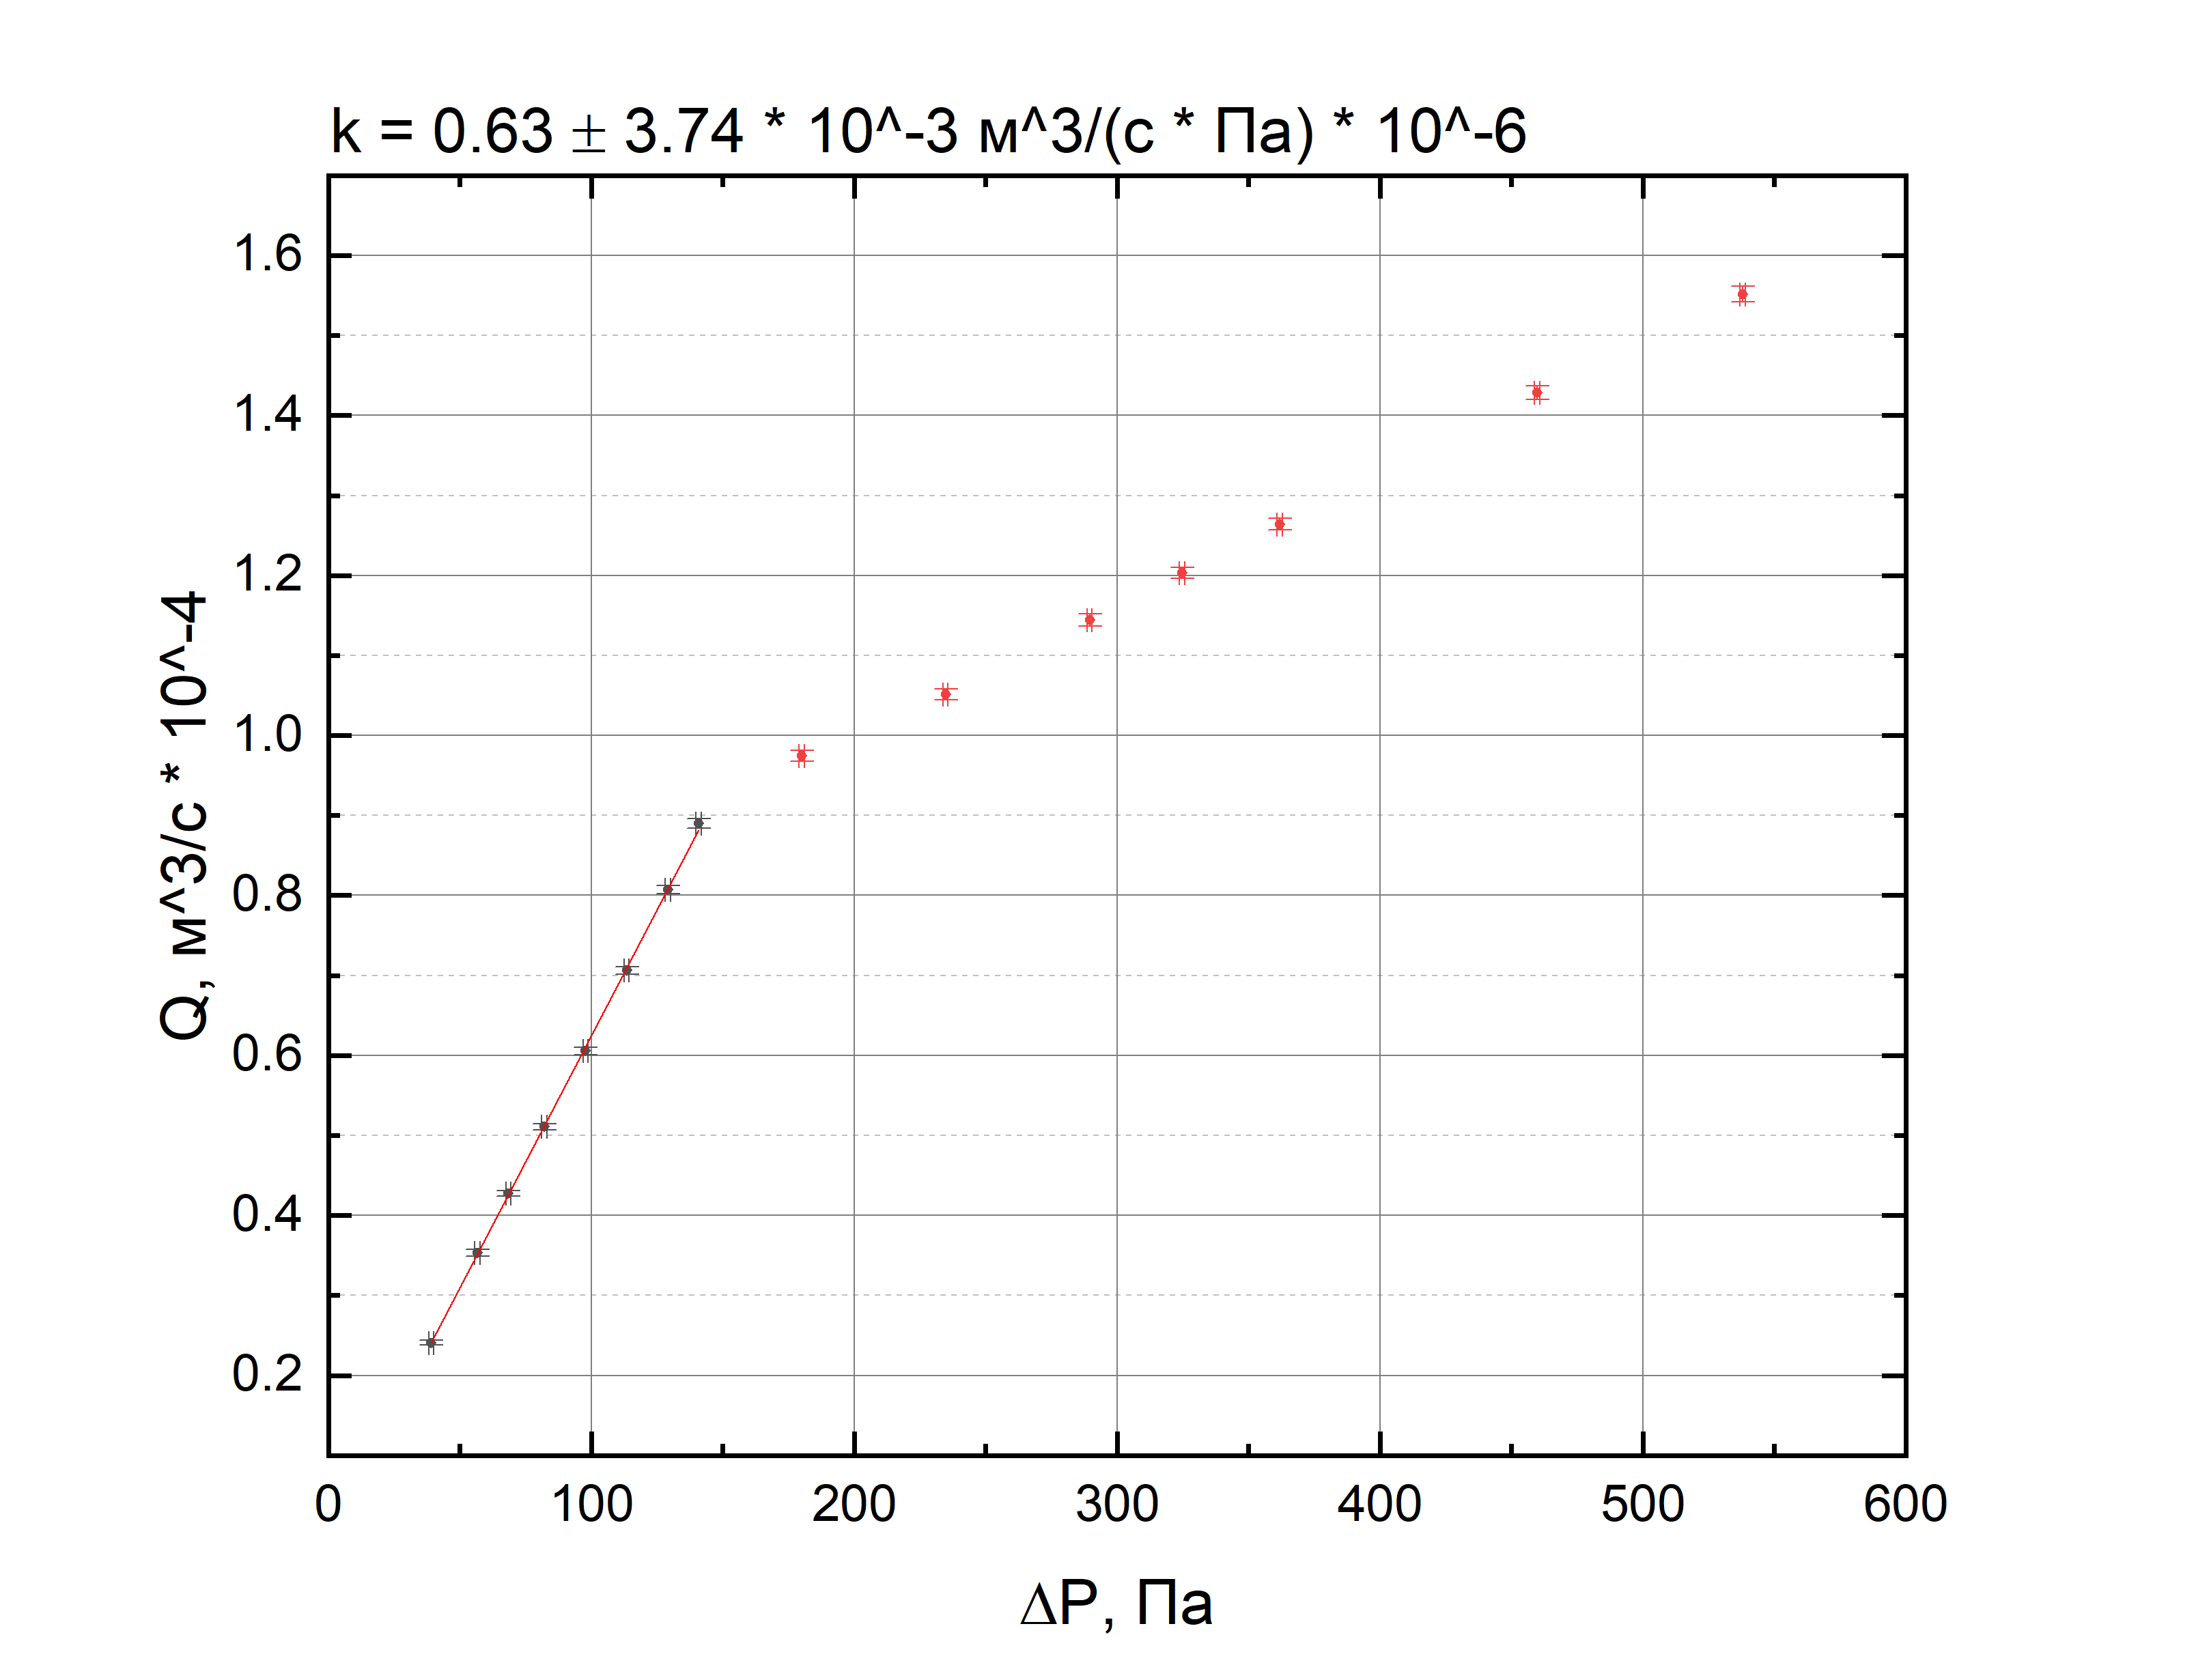
\includegraphics[width=0.83\textwidth]{G1.jpg}
    \caption{График для $d = 3,95$ мм}
\end{figure}

\begin{figure}[!ht]
    \centering
    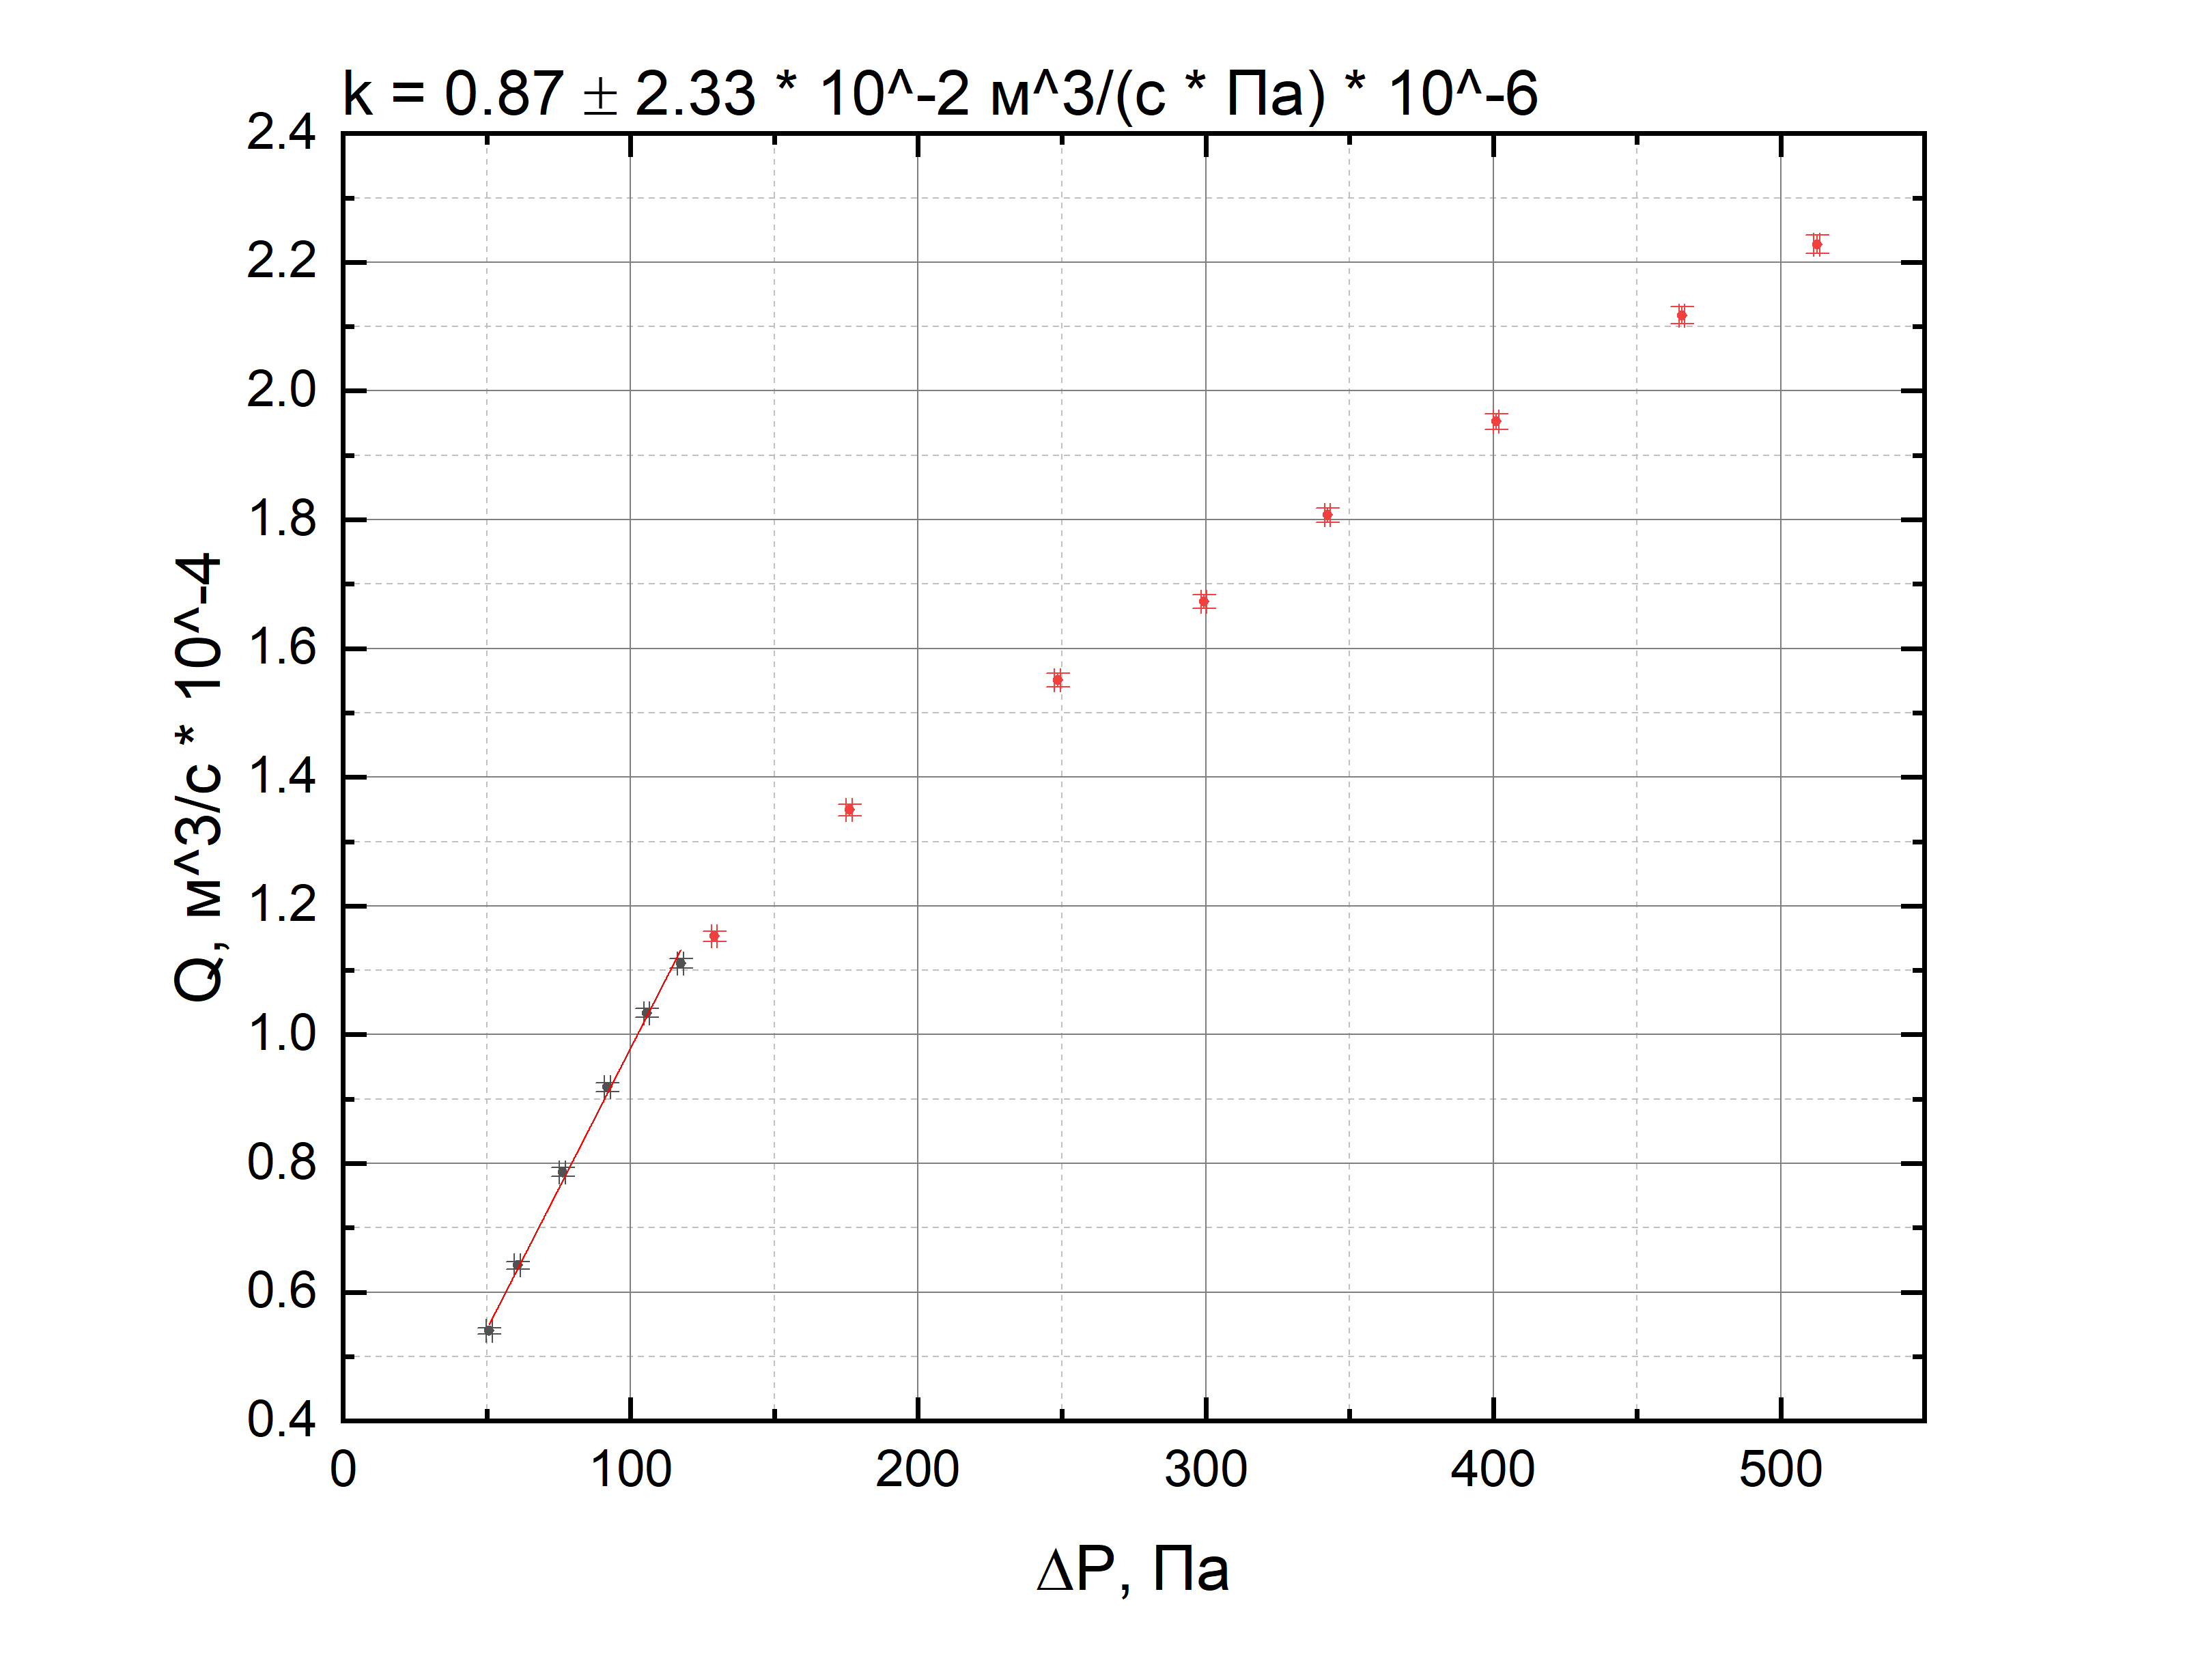
\includegraphics[width=0.83\textwidth]{G2.jpg}
    \caption{График для $d = 5,05$ мм}
\end{figure}

\begin{figure}[!ht]
    \centering
    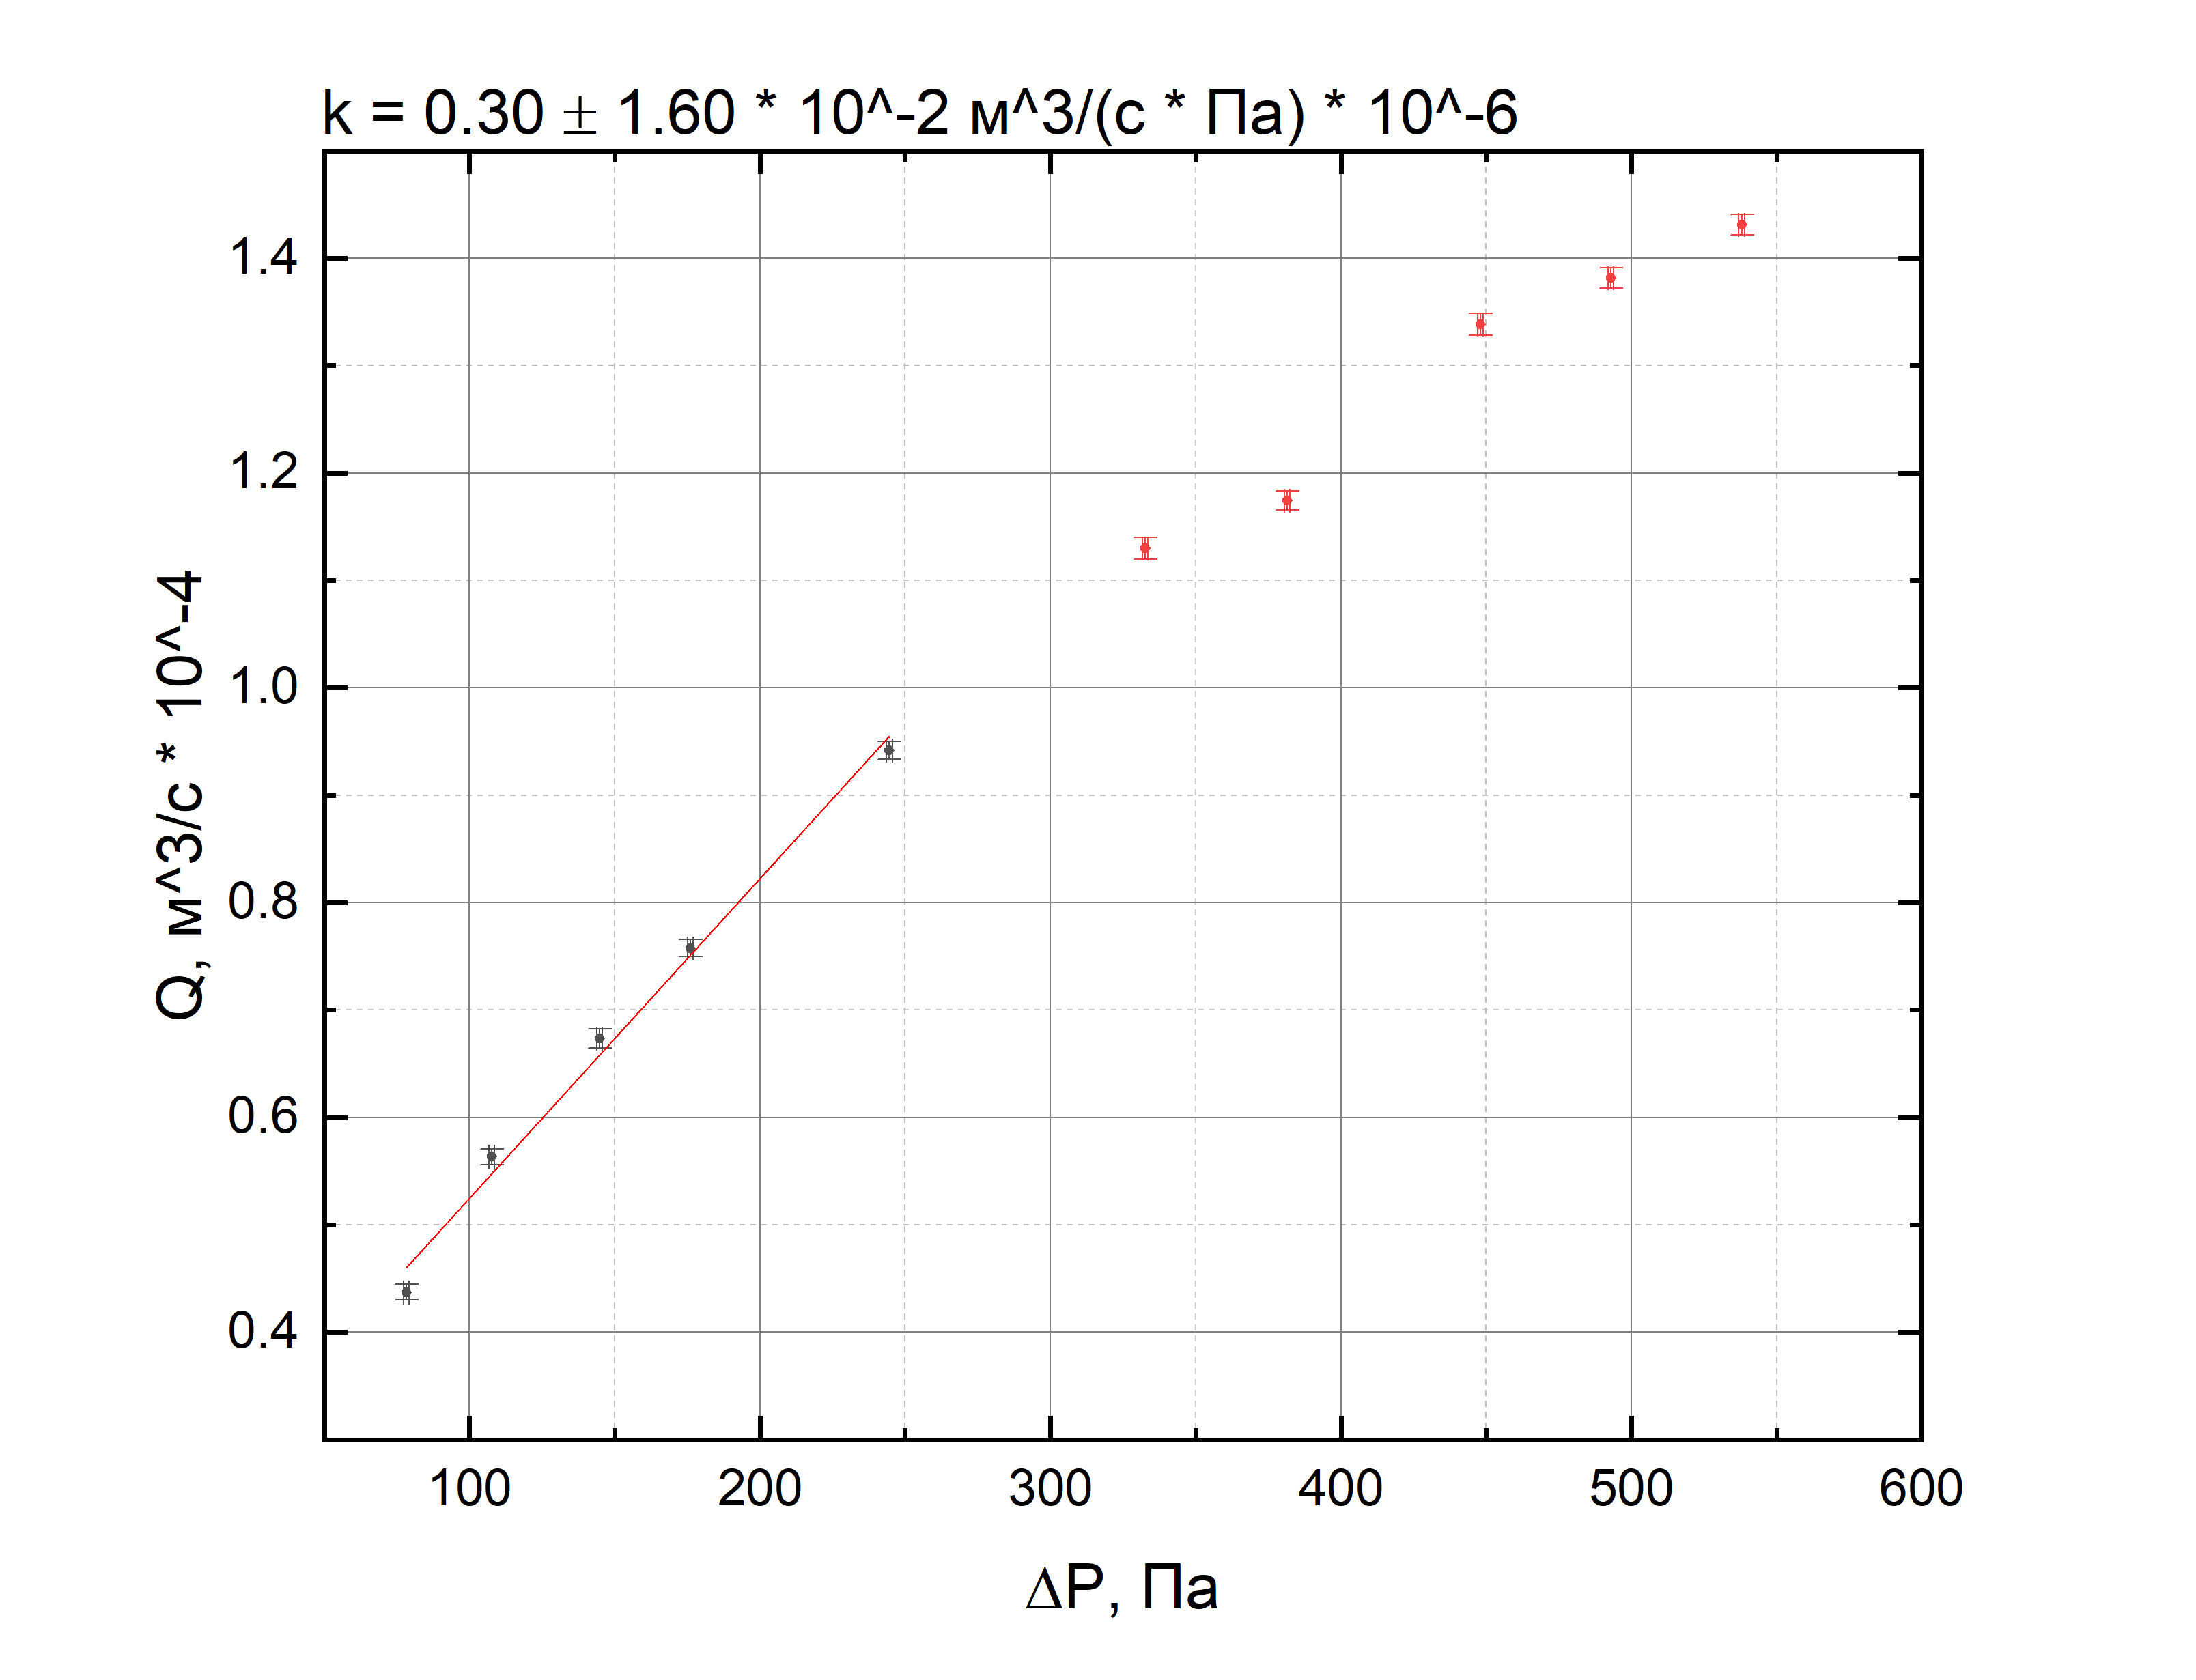
\includegraphics[width=0.83\textwidth]{G3.jpg}
    \caption{График для $d = 3$ мм}
\end{figure}

Линии проведены при помощи МНК, по точкам с ламинарным течением.
	
	С помощью коэффициентов наклона мы можем найти вязкость воздуха из формулы (3):
	
	\begin{equation*}
		\eta = \frac{\pi R^4}{8kl}
	\end{equation*}
	где $k$ -- коэффициент наклона графика, $l$ -- длина участка трубы, а $R$ -- радиус трубки.
	
	По графикам определим значения коэффициента наклона с погрешностями:

	\begin{table}[!ht]
		\begin{center}
		\bgroup
		\def\arraystretch{1.1}%
			\begin{tabular}{|c|c|c|c|}
				\hline
				&$d_1 = 3.0$ мм&$d_2 = 3.95$ мм&$d_3 = 5.05$ мм\\ \hline
				$k\cdot10^{-6}$, $\text{м}^3$/с$\cdot$Па& 0,3 & 0,63 & 0,87\\ \hline
				$\sigma_k \cdot10^{-6} $ , $\text{м}^3$/с$\cdot$Па& 0.02 & 0.004 & 0,02 \\ \hline
				$\eta\cdot10^{-5}$, Па$\cdot$с&1.66&1.90&2,04 \\ \hline
				$\sigma_\eta\cdot10^{-5}$, Па$\cdot$с&0.11&0.01&0.05\\ \hline
			\end{tabular}
		\egroup
		\caption{Результаты полученные из графиков}
		\end{center}
	\end{table}
    Возьмем два последних значения и усредним
	
    \begin{equation*}
		\eta = (1.97\pm 0.03) \cdot 10^{-5} \text{ Па}\cdot \text{с}
	\end{equation*} 
	
	Далее найдем критическое число Рейнольдса $Re_\text{кр}$ для всех трубок:
	\begin{equation*}
		Re = \frac{\rho u R}{\eta} = \frac{\rho Q}{\pi R \eta}
	\end{equation*}
	\begin{itemize}
		\item $d_1 = 3.00$ мм: критический расход: $Q_1 = 0,94\cdot10^{-4}\text{ м}^3$/c, тогда $Re_1 = 1143 \pm 20.$
		\item $d_2 = 3.95$ мм: критический расход: $Q_2 = 0,89\cdot10^{-4}\text{ м}^3$/c, тогда $Re_2 = 870 \pm 15.$  
		\item $d_3 = 5.05$ мм: критический расход: $Q_3 = 1,11\cdot10^{-4}\text{ м}^3$/c, тогда $Re_3 =  854\pm 14.$ 
	\end{itemize}

    \subsection*{Распределение давления газа вдоль трубки}

    Установили поток воздуха через трубку, близкий к критическому, но все еще сохраняющий ламинарный. Не меняя формат, подсоединим микроманометр ко всем выводам и измерим перепады давления. 

    \begin{table}[!ht]
        \centering
        \begin{tabular}{|c|c|c|c|c|}
        \hline
            $d, мм$ & $Q$ м$^3$/c $\cdot$ 10$^{-4}$ & $L$, см & $p$, дел. & $p$, Па \\ \hline
            3,95 & 0,084 & 50 & 68 & 133,3 \\ \hline
            3,95 & 0,084 & 90 & 125 & 245,0 \\ \hline
            3,95 & 0,084 & 120 & 220 & 431,2 \\ \hline
            5,05 & 0,11 & 90 & 59 & 115,6 \\ \hline
            5,05 & 0,11 & 120 & 77 & 150,9 \\ \hline
        \end{tabular}
        \caption{Полученные данные}
    \end{table}

    Построим полученные графики 


    \begin{figure}[!ht]
        \centering
        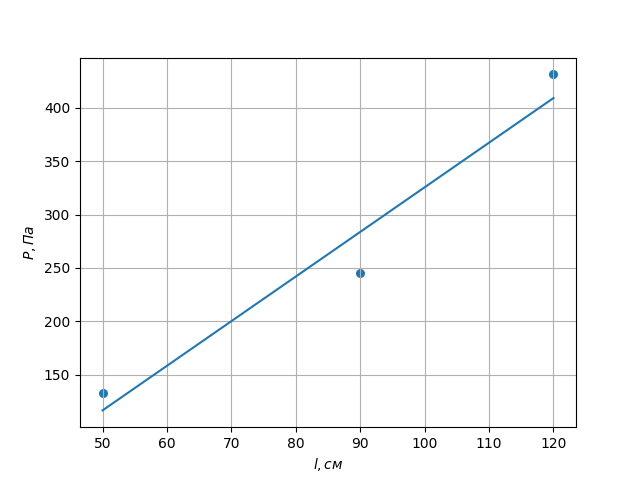
\includegraphics[width=0.83\textwidth]{first.png}
        \caption{График для $d = 3,95$ мм}
    \end{figure}

    \begin{figure}[!ht]
        \centering
        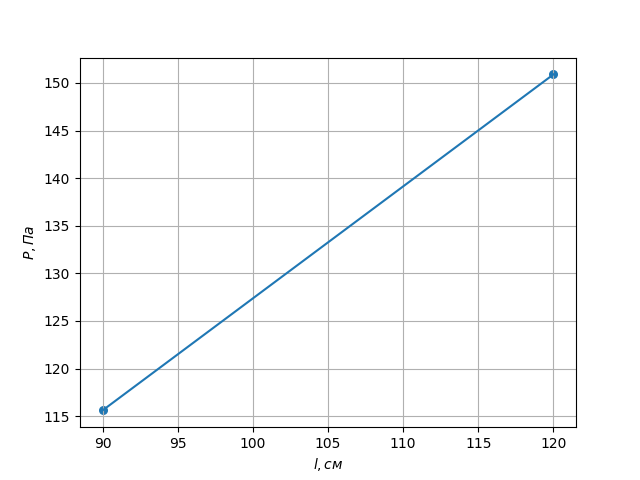
\includegraphics[width=0.7\textwidth]{second.png}
        \caption{График для $d = 5,05$ мм}
    \end{figure}

    \subsection*{Измерение зависимости расхода от радиуса трубы при заданном градиенте}

    Подобрали некоторое значение градиента давления, при котором на всех трубках происходит ламинарное течение воздуха. Для каждой трубки подобрали расход, когда градиент равен данному. $\Delta P / l = 0,72$ дел/см

    \begin{table}[!ht]
        \centering
        \begin{tabular}{|c|c|c|c|c|c|c|c|}
        \hline
            $l$, см & $P$, дел. & $d$, мм & ln(r) & $V$, л & $t$, c & $Q$ м$^3$/c $\cdot$ 10$^{-4}$ & ln(Q) \\ \hline
            90 & 65 & 5,05 & 0,93 & 6 & 52,69 & 0,11 & -2,17 \\ \hline
            40 & 29 & 3 & 0,41 & 2 & 63,3 & 0,03 & -3,45 \\ \hline
            50 & 36 & 3,95 & 0,68 & 4 & 75,9 & 0,05 & -2,94 \\ \hline
        \end{tabular}
        \caption{Полученные данные}
    \end{table}
    
    \begin{figure}[!ht]
        \centering
        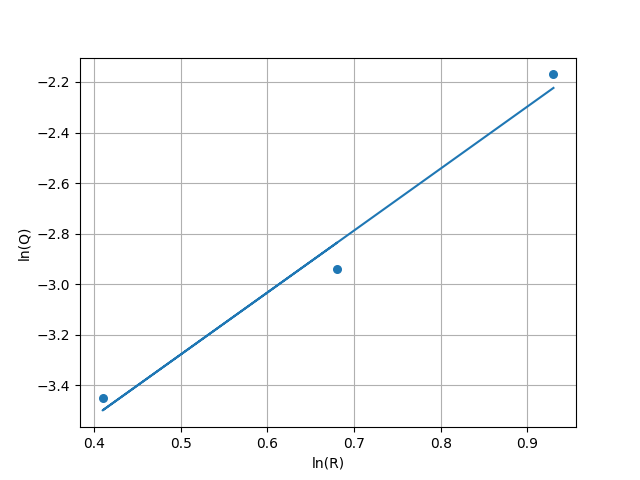
\includegraphics[width=0.7\textwidth]{ln.png}
        \caption{График для определение степени $\beta$ }
    \end{figure}

По МНК получим, что для ламинарного течения $ \beta = 2,45 \pm 0,37 $.

\section{Вывод}

В данной лабораторной работе мы исследовали свойства течения газов по тонким трубам при различных числах Рейнольдса. Так же выявили область применимости закона Пуазейля и с его помощью определили коэффициент вязкости воздуха. 
\[ \eta = (1.97\pm 0.09) \cdot 10^{-5} \text{ Па}\cdot \text{с} \] 

Сравним с табличным значением которое равно

\[ \eta = 1.78 \cdot 10^{-5} \text{ Па}\cdot \text{с} \] 

Видно, что значения получились довольно близки друг к другу. Малое расхождение обусловлено тем, что в этой лабораторной работе нет приборов, которое бы вносило большую погрешность, а объем и время мы мерили так, чтобы относительная погрешность расхода была меньше процента. 

Также в работе была изучена зависимость расхода от радиуса трубы при заданном градиенте. Для ламирного течения мы получили показатель степени $2.45$, что должно быть показателем степени для турбулентного течения. Возможно, мы неправильно посчитали градиент, и в каждой трубке было турбулентное течение.

\end{document}